\subsection{Adiabatic perturbations}\label{analytic_adia}
We now consider % general $\gamma$
perturbations in the adiabatic limit ($t_c,\beta\to\infty$). This is the opposite regime to
isothermal perturbations. In this case the parameter $\chi = 1/\gamma$
and Eq. \ref{vertiso_gov_nondim} can be written as 
% We eliminate variables from 
% Eq. \ref{lin_mass}---\ref{lin_energy} in favor of $\delta v_z$ 
% and $\Delta \equiv \nabla\cdot\delta\bm{v}$ to obtain
% \begin{align}
%   &\Delta\left(1 + \frac{\gamma c_s^2 k_x^2}{D}\right) = \frac{d\delta
%     v_z}{dz} + \frac{\ii k_x^2}{D}\left(\ii c_s^2 \frac{d\ln\rho}{dz}
%     - \frac{r}{k_x}\frac{d\Omega^2}{dz}\right)\delta v_z,\label{adia_iso1}\\
%   & -\frac{\sigma^2}{c_s^2}\delta v_z = \gamma \frac{d\Delta}{dz} +
%   \frac{d}{dz}\left(\frac{d\ln\rho}{dz}\delta v_z\right) +
%   \left(\gamma-1\right)\frac{d\ln\rho}{dz} \Delta.\label{adia_iso2}
% \end{align}
% %{\bf note: incompressible mode, set delta to zero. only works for
% % constant gravity.}

% We make the low-frequency approximation and the replacement 
% $D\to \Omega_k^2$ in Eq. \ref{adia_iso1}---\ref{adia_iso2}. For
% simplicity we do this before combining these equations later. We  
% show in Appendix \ref{adia_improve} that making these approximations
% after combining  Eq. \ref{adia_iso1}---\ref{adia_iso2} adds unecessary
% complexity for thin disks. Here, we also use the fact that in the
% global disk, 
% \begin{align}
%   r\frac{\p \Omega^2}{\p z} = -\frac{\p \ln\rho}{\p z} \frac{qc_s^2}{r},
% \end{align}
% for the power-law prescription of the midplane sound-speed for
% $\Gamma=1$.  

% Making the above substitutions and eliminating $\Delta$ between Eq. \ref{adia_iso1}---
% Eq. \ref{adia_iso2} we obtain, in terms of dimensionless variables defined
% previously, an equation for $\delta v_z$, 

\begin{align}
  0 =& \dd v_z^{\prime\prime} + \left(1 + \ii \epsilon q
    \hat{k}\right)\left(\ln\rho^{\prime}\delta v_z\right)^\prime\notag\\
  &+\left\{\hat{\sigma}^2\left(\frac{1}{\gamma}+\hat{k}^2\right)\right.\notag\\
  &\phantom{0=}\left.-\left(\frac{\gamma-1}{\gamma}\right)\left[\ln\rho^{\prime\prime}+\hat{k}^2\left(1-\frac{\ii\epsilon  
          q}{\hat{k}}\right)\ln\rho^{\prime 2}\right]\right\}\delta v_z.\label{adia_iso3}
\end{align}

We multiply Eq. \ref{adia_iso3} by $\rho\delta v_z^*$ and
integrate vertically, assume boundary terms vanish when integrating by
parts, to obtain
\begin{align}
  &\hat{\sigma}^2\left(\frac{1}{\gamma} +
    \hat{k}^2\right)\int_{\zhat_1}^{\zhat_2}\rho|\delta
  v_z|^2 d\zhat \notag\\
  &=  \left(\frac{\gamma-1}{\gamma}\right)
  \int_{\zhat_1}^{\zhat_2}\rho|\delta v_z^\prime|^2 d\zhat
  +\frac{1}{\gamma}\int_{\zhat_1}^{\zhat_2}\frac{1}{\rho}|(\rho\delta
  v_z)^\prime|^2 d\zhat\notag\\
  &\phantom{=} +
  \left(\frac{\gamma-1}{\gamma}\right)\hat{k}^2\left(1-\frac{\ii\epsilon
      q}{\hat{k}}\right) \int_{\zhat_1}^{\zhat_2}\rho\ln\rho^{\prime
    2}|\delta v_z|^2 d\zhat\notag\\
  &\phantom{=} + \ii\epsilon q \hat{k}
  \int_{\zhat_1}^{\zhat_2}\ln\rho^\prime(\rho\delta v_z^*)^\prime
  \delta v_z d\zhat.\label{adia_integral}
\end{align}
When $q\equiv0$, all the terms on the right-hand-side (RHS) are real. Then
$\hat{\sigma}^2$ is real, and  $\hat{\sigma}^2>0$ if $\gamma>1$. As
expected, a sub-adiabatically stratified disk is stable in the absense
of vertical shear. In the presence of vertical shear $q\neq0$ and
$\hat{\sigma}$ is generally complex, which implies the possibility of
instability.  

Note that when $\gamma>1$ and $q=0$, the term with $\ln\rho^{\prime
  2}$ in the integrand (third term on the RHS) represents
stabilization by the vertical entropy gradient (real buoyancy frequency). 
It gives an imaginary contribution to $\hat{\sigma}$ when $q\neq0$,
but this is a factor $|\epsilon/\hat{k}|$ smaller than the real
(stabilizing) contribution, 
since $\epsilon\ll 1$ for a thin disk and we (usually) consider
$\hat{k}\gg1$. Thus, instability is expected to be associated with the 
last term on the RHS of Eq. \ref{adia_integral}. 

\subsubsection{Explicit solutions in the thin-disk limit}\label{adia_explicit}
We can construct solutions in the thin-disk limit, in which 
$\ln(\rho/\rho_0) \simeq -\zhat^2/2$. Eq. \ref{adia_iso3} becomes   
\begin{align}
  0 = \delta v_z^{\prime\prime} - \zhat A \delta v_z^\prime + \left(B
    - C \zhat^2\right)\delta v_z, \label{adia_iso4} 
\end{align}
with
\begin{align}
  &A \equiv 1 + \ii \epsilon q \hat{k},\\
  &B \equiv \hat{\sigma}^2\left(\frac{1}{\gamma} + \hat{k}^2\right) -
  \left(\frac{1}{\gamma} + \ii \hat{k} \epsilon q\right)\\
  &C \equiv \frac{\left(\gamma-1\right)}{\gamma}\hat{k}^2\left(1 - \frac{\ii
      \epsilon q}{\hat{k}}\right).\label{adia_thin}
\end{align}
Let
\begin{align}
  \delta v_z(\zhat) =
  g(\zhat)\exp\left(\frac{\alpha\zhat^2}{2}\right), \label{adia_ansatz}
\end{align}
where $\alpha$ is a constant to be chosen for convenience. Inserting
Eq. \ref{adia_ansatz} into Eq. \ref{adia_thin} gives
\begin{align}
  0 = g^{\prime\prime} - \hat{z}\left(A - 2\alpha\right)g^\prime + \left(B +
    \alpha\right)g
  +\left(\alpha^2 - \alpha A - C\right)\zhat^2 g.
\end{align}
We choose $\alpha$ to make the coefficient of $\zhat^2g$
vanish, and impose the vertical kinetic energy density
$\rho|\delta v_z|^2$ to remain finite. Then assuming $g(\zhat)$ is a
polynomial, we require  
\begin{align}
  \real\alpha < \frac{1}{2}. 
\end{align}
We therefore choose 
\begin{align}
  \alpha = \frac{1}{2}\left(A - \sqrt{A^2 + 4C}\right). 
\end{align} 

We now have an equation in the same form as Eq. \ref{iso_ode3}:
\begin{align}
  0 = g^{\prime\prime} - \hat{z}\left(A - 2\alpha\right)g^\prime +
  \left(B + \alpha\right)g.
\end{align}
We seek polynomial solutions 
\begin{align}
  g(\zhat) = \sum_{m=0}^M b_m \zhat^m,
\end{align}
% We again seek power-series solutions 
% \begin{align}
%   g(\zhat) = \sum_{m=0}^\infty b_m \zhat^m,
% \end{align}
% which requires
% \begin{align}
%   (m+2)(m+1)b_{m+2} + \left[\left(2\alpha - A\right)m + B + \alpha\right]=0.
% \end{align}
which requires
\begin{align}
  B + \alpha = M\left(A-2\alpha\right).\label{adia_disp0}
\end{align}
Inserting the definition of $B$ we get
\begin{align}
  &\hat{\sigma}^2\left(\frac{1}{\gamma}+\hat{k}^2\right) \notag\\ &=
  \left(\frac{1}{\gamma}-\frac{1}{2}\right) +\frac{\ii}{2}\epsilon q
  \hat{k} + \frac{1}{2}\left(2M+1\right)\left(A^2 + 4C\right)^{1/2}\label{adia_disp}. 
\end{align}
This gives the eigenfrequency $\hat{\sigma}$ and completes the solution
description.  

%Recalling that $B$ depends $\hat{\sigma}$, Eq. \ref{adia_disp} gives
%the eigenfrequency as a function of disk paramters. 

\subsubsection{The case of $\gamma=2$}
In principle, we can solve Eq. \ref{adia_disp} for the mode
frequencies and growth rates as a function of the disk parameters and
the radial wavenumber. This is complicated in 
general, but simplifies for $\gamma=2$, for which the quantity
$A^2+4C$ is real. In this case we find
\begin{align}
  \hat{\nu}^2 =
  \frac{1}{2}\frac{(2M+1)}{\sqrt{1+2\hat{k}^2}}&\left[
    \sqrt{1-\frac{4M(M+1)\hat{k}^2\epsilon^2q^2}{(2M+1)^2(1+2\hat{k}^2)}}\right.\notag\\
  &\phantom{=}
  \left.- \sqrt{1 - \frac{\hat{k}^2\epsilon^2q^2}{(1+2\hat{k}^2)}}\right].
\end{align}
In the limit of a thin disk $\epsilon\to0$ or weak shear $|q|\to0$, we
have 
\begin{align}
  \hat{\nu}^2 = \frac{\epsilon^2
    q^2}{4(2M+1)}\frac{\hat{k}^2}{(1+2\hat{k}^2)^{3/2}},\label{gam2_growth}
\end{align}
and the maximum growth rate occurs at $\hat{k}=\hat{k}_\mathrm{opt}=1$,  
\begin{align}
  \mathrm{max}(\hat{\nu}) &= \frac{|\epsilon
    q|}{2(3^{3/4}\sqrt{2M+1})}\label{gam2_max_growth}.
  % & \leq \frac{|\epsilon
  % q|}{2\times3^{3/4}}\notag.
\end{align}
Unlike isothermal perturbations, Eq. \ref{gam2_max_growth} shows that
maximum growth rate occurs at $M=0$, and growth rates decrease with increasing $M$. This
is despite the fact that in the thin-disk approximation 
$d\Omega^2/dz\propto z$, so there is infinite vertical shear
available.     

The acceptable solution for $\alpha$ when $\gamma=2$ is
\begin{align}
  \alpha = \frac{1}{2}\left[\left(1+\ii\epsilon q \hat{k}\right) -
    \sqrt{1 + \hat{k}^2\left(2-\epsilon^2 q^2\right)}\right].\label{gam2_alpha}
\end{align}
Since $\epsilon\ll 1$, $\real\alpha<0$, so the vertical velocity
eventually decays for large heights. For $\hat{k}\gg 1$ the
perturbation decays rapidly away from the midplane. This is again
unlike isothermal perturbations, whose magnitude increase with $|z|$.  

%gauss decay means boundary conditions have no influence, all perts go
%to zero

\subsubsection{Comparison with $\gamma=1$}\label{adia_compare_gam1}
We can compare growth rates obtained for $\gamma=2$ to those for
$\gamma=1$ in the previous section. If we compare growth rates at their 
respective optimum radial wavelengths, we find
that for $\gamma=2$ the \emph{maximum} growth rate, occuring
at $M=0$, is still $\sim2$ times smaller than the \emph{minimum} growth
rate for $\gamma=1$. That is,
\begin{align}
  &\mathrm{max}(\hat{\nu}) \geq \frac{|\epsilon q|}{2\sqrt{1+|\epsilon
      q|}} & \text{at }\hat{k} = \hat{k}_\mathrm{opt} \text{ for }   \gamma=1,  \\
  &\mathrm{max}(\hat{\nu}) \leq \frac{|\epsilon q|}{2\times 3^{3/4}}
           & \text{at }\hat{k} = \hat{k}_\mathrm{opt} \text{ for } \gamma=2.
\end{align}

We can also compare growth rates in the limit $\hat{k}\gg1$ using
Eq. \ref{simple_growth} and Eq. \ref{gam2_growth},
\begin{align}
  &\hat{\nu} \geq \sqrt{\frac{|\epsilon q|}{2\hat{k}}}
  &  \text{as }  \hat{k}\to\infty  \text{ for }  \gamma=1, \\
  &\hat{\nu} \leq \frac{|\epsilon q|}{2^{7/4}\sqrt{\hat{k}}}
  &\text{as }  \hat{k}\to\infty  \text{ for }  \gamma=2.\label{gam2_growth_rate}
\end{align}
Then the growth rate of perturbations with large $|\hat{k}|$ in a
$\gamma=2$ disk is at most $2^{-5/4}\sqrt{|\epsilon q|}$ times that in a
$\gamma=1$ disk. For $\epsilon = 0.1$ and $|q|=1$, this factor is
$\sim 0.1$.  

In Fig. \ref{adia_growth} we plot the eigenfrequencies as a
function of the radial wavenumber $\hat{k}$, for a range of adiabatic
indices, using Eq. \ref{adia_disp}. The low-frequency approximation
is questionable for $\hat{k}\lesssim4$ since
$|\hat{\sigma}|^2\gtrsim0.2$. For large $\hat{k}$ the presence of a
positive vertical entropy gradient is strongly stabilizing. This is
because the vertical shear grows as $z$ away from the midplane (and
has a maximum when the thin-disk approximation is relaxed), but square
of the bouyancy frequency, which is stabilizing, grows as $z^2$ away
from the midplane. %The entropy $P/\rho^\gamma$ formally diverges   
%for $z\to\infty$ even without the thin-disk approximation.        

\begin{figure}
  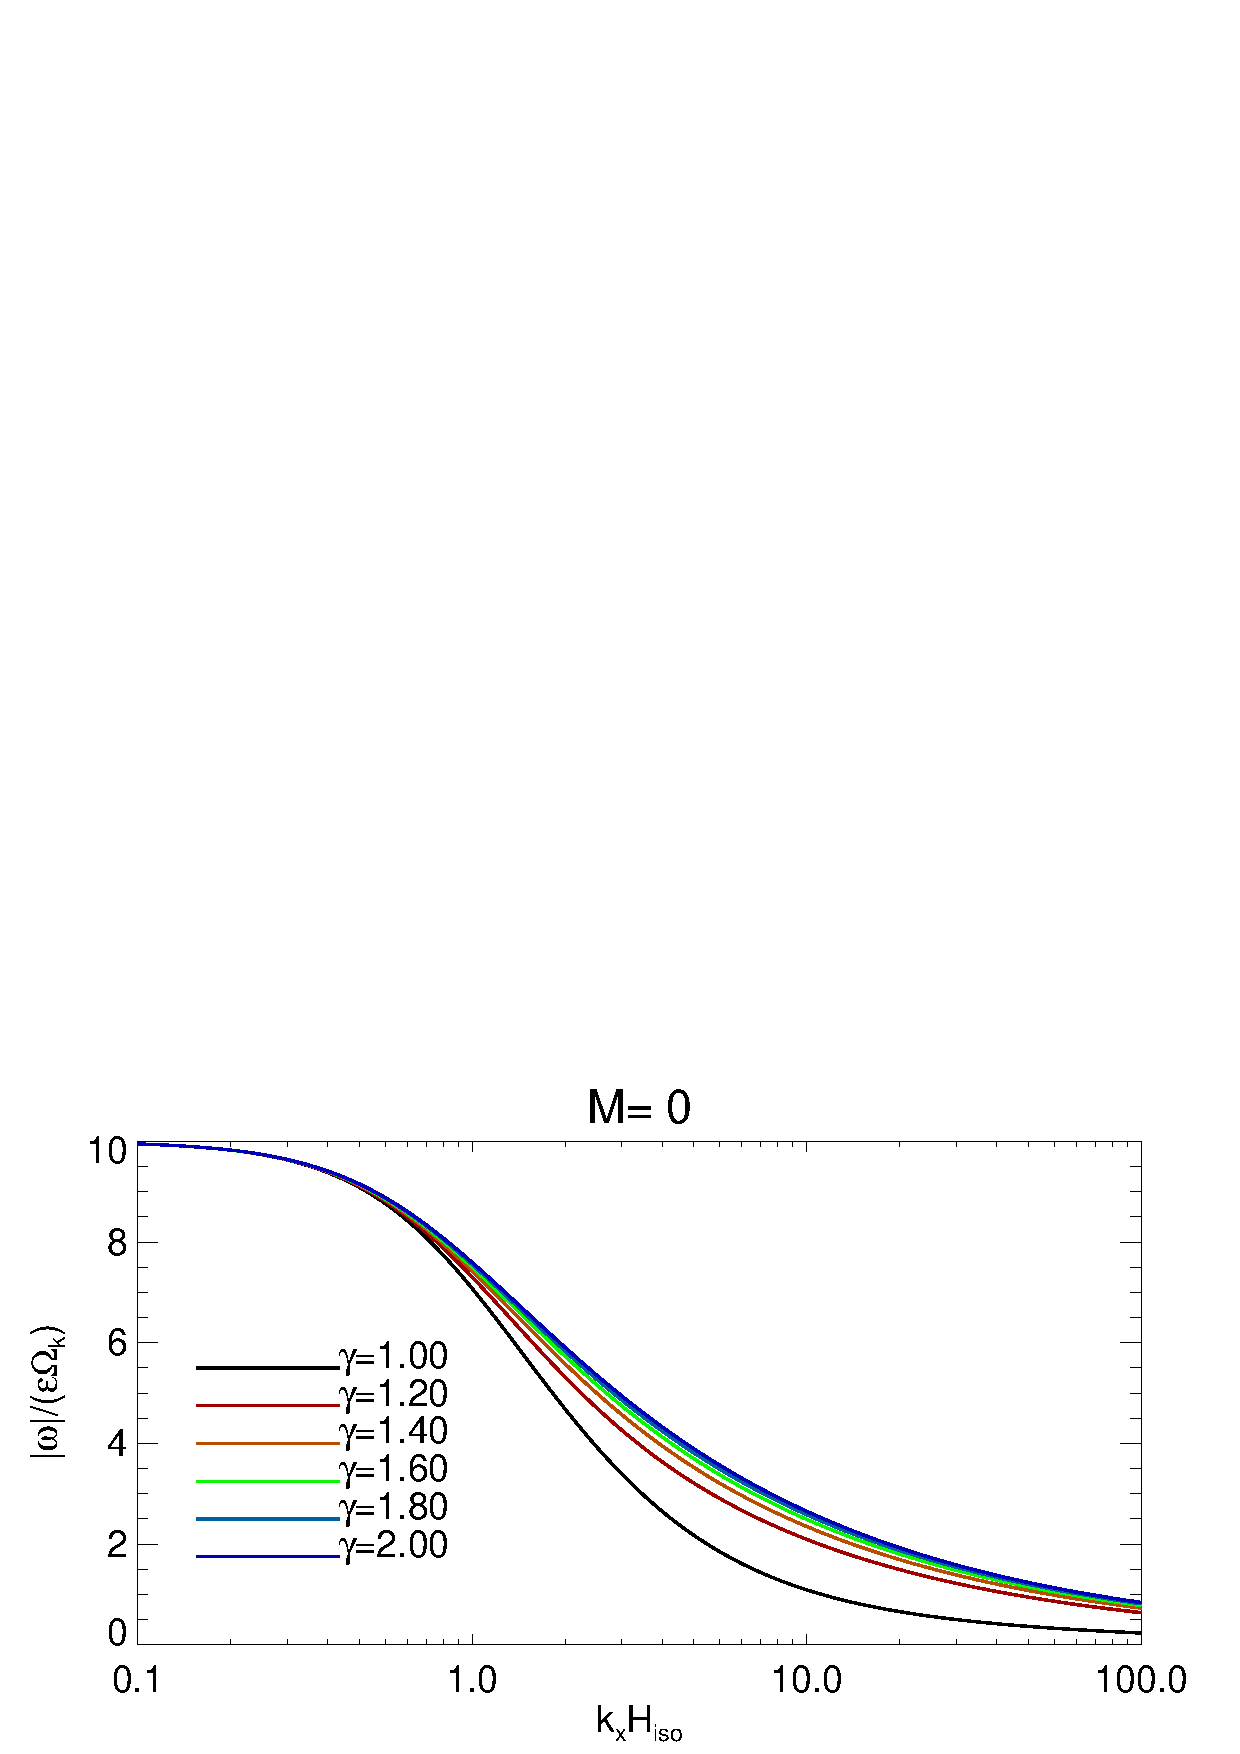
\includegraphics[width=\linewidth,clip=true,trim=0cm 1.75cm 0cm 0cm]{figures/rate_theory_om}
  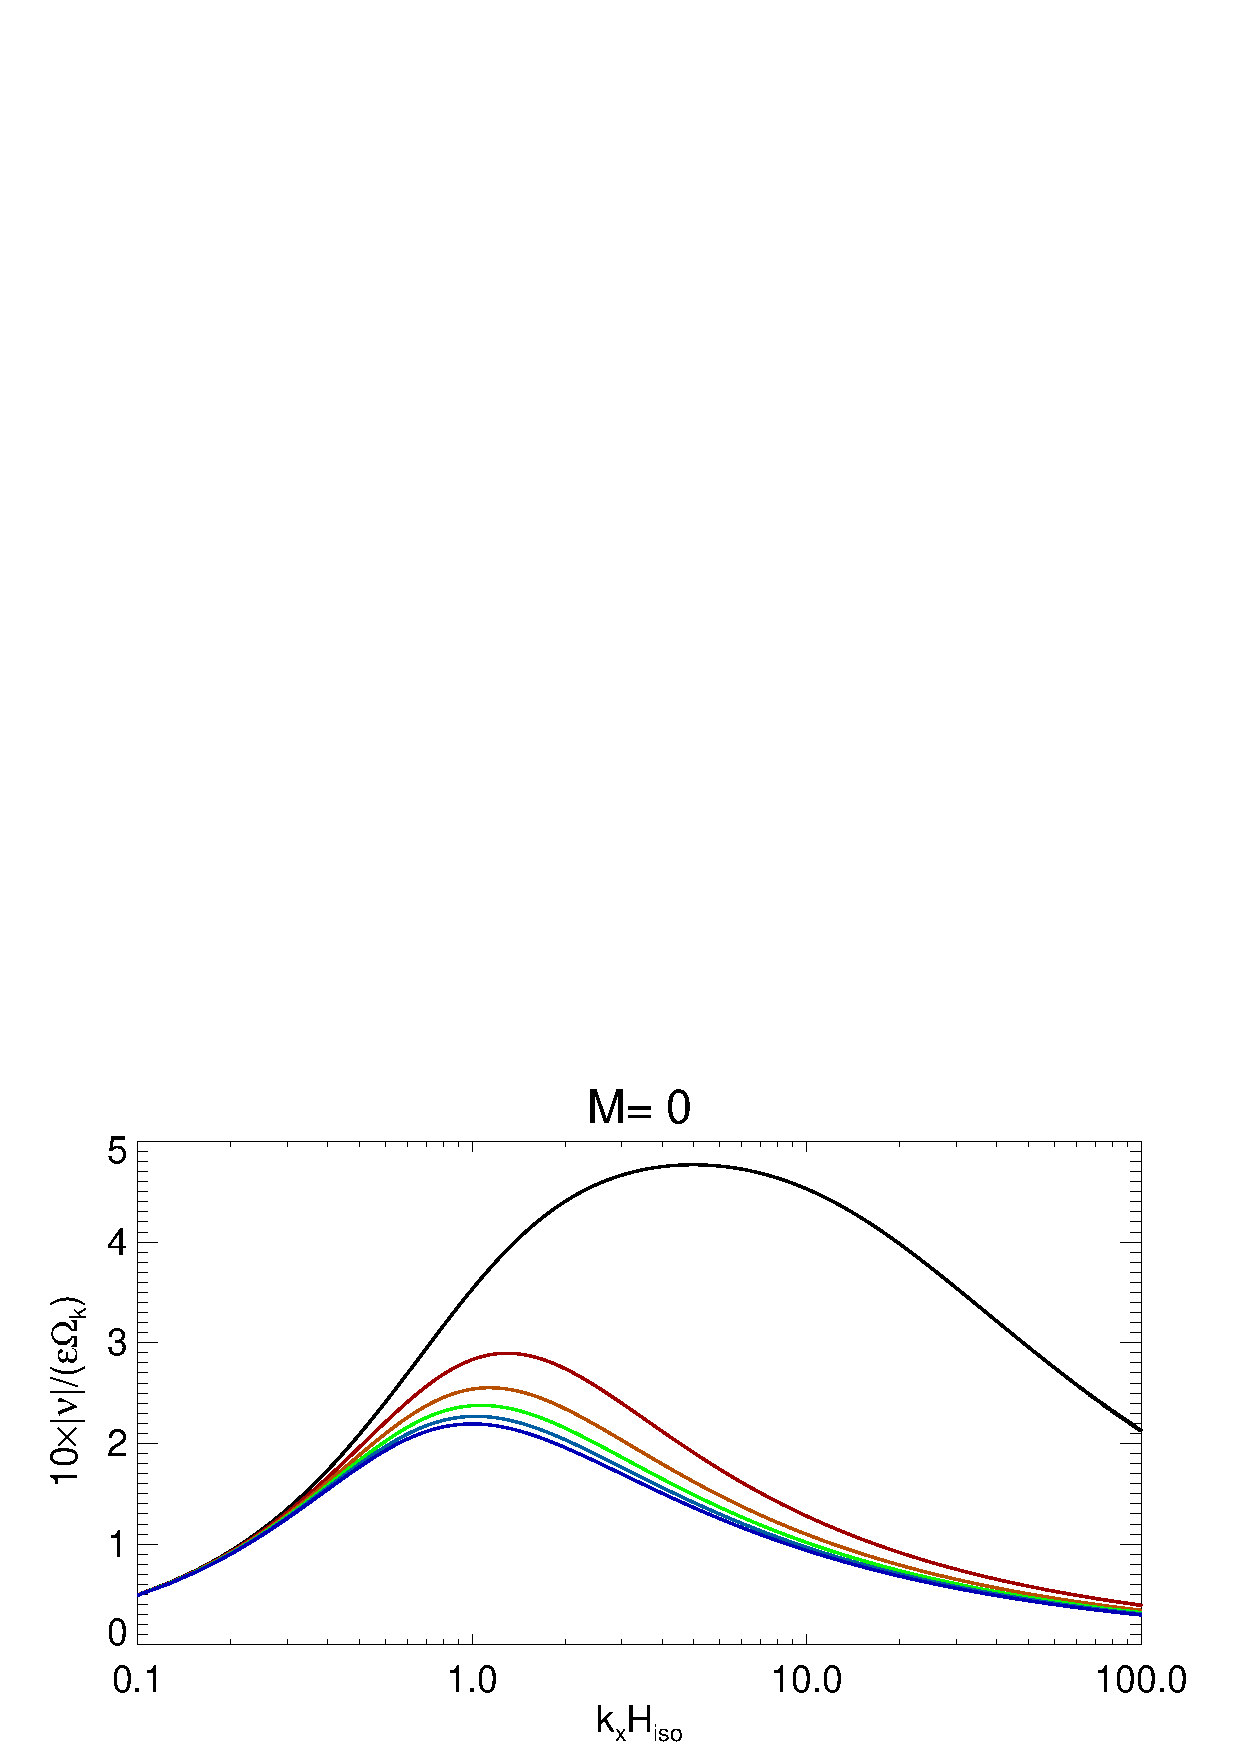
\includegraphics[width=\linewidth,clip=true,trim=0cm 0cm 0cm 1cm]{figures/rate_theory_nu}
  \caption{Real frequency (top) and growth rate (bottom) of the fundamental VSI mode in vertically 
    isothermal disks ($\Gamma=1$) subject to adiabatic perturbations,
    calculated in thin disk approximation from Eq. \ref{adia_disp}
    with $M=0$, $\epsilon=0.1$ and  
    $|q|=1$. Frequencies are shown as a function of the radial
    wavenumber for different values of the adiabatic index
    $\gamma$. For $\gamma\equiv 1$ the perturbations are isothermal
    and there is no vertical entropy gradient.\label{adia_growth}}  
\end{figure}   

% \subsubsection{Qualitative condition for buoyancy to be negligible in
%   the presence of thermal relaxation}
% {\bf this section might be wrong, but keep for reference for now}
% We have shown that when $\gamma>1$ so that there is a positive
% vertical entropy gradient and perturbations evolve
% adiabatically ($t_c\to\infty$) that the VSI is strongly
% surpressed. This is the limit where the term proportional to
% $t_c^{-1}$ in the linearized energy equation (Eq. \ref{lin_energy})
% becomes negligible compared to the term proportional to
% $\gamma/\Gamma-1$. The latter term is associated with the vertical
% entropy gradient, or buoyancy frequency squared, $N_z^2$. 

% Reversing the argument, we expect to recover the VSI when the bouyancy
% frequency becomes negligible compared to the cooling rate, or 
% \begin{align}
%   t_c \ll \frac{\Omega}{\gamma N_z^2}. 
% \end{align} 
% Parametrizing $t_c = \beta\Omega_k^{-1}$ and inserting the expression
% for $N_z^2$ appropriate for vertically isothermal disks, we expect
% \begin{align}
%   \beta \ll
%   \frac{1}{H^2_\mathrm{iso}\left(\gamma-1\right)\left(\frac{\p\ln\rho}{\p
%           z}\right)^2} 
% \end{align}
% is required to enable the VSI, where we used $\Omega\sim\Omega_k$.  
% This inequality is satisfied at the
% midplane and as $|z|\to\infty$. It can be satisifed at all heights if
% it is satisfied at the height of $\mathrm{max}|\p\ln\rho/\p z|$. 
% Using the full expression for the density field for vertically isothermal
% disks (Eq. \ref{vertiso_eqm}), we expect 
% \begin{align}
%   \beta \ll \frac{27}{4(\gamma-1)}\epsilon^2,
% \end{align}
% i.e. $\beta\ll O(\epsilon^2)$, is a sufficient condition for
% buoyancy to be negligible. 

\subsection{Perturbations with thermal relaxation}\label{analytic_relax}
Having examined the extreme limits of isothermal ($t_c\to0$) and
adiabatic ($t_c\to\infty$) perturbations, we now generalize further to consider
perturbations with intermediate thermodynamic responses with general
values of $t_c$ or $\beta$.  

In this section we will pursue explicit solutions in the thin-disk
approximation. The governing equation, Eq. \ref{vertiso_gov_nondim}, is
then 
\begin{align}
  0 = \delta v_z^{\prime\prime} - z \widetilde{A}\delta v_z^\prime +
  (\widetilde{B} - \widetilde{C}\zhat^2)\delta v_z = 0,\label{nearly_iso_explicit}
\end{align}
with
\begin{align}
  &\widetilde{A} \equiv 1 + \ii \epsilon q \hat{k},\\
  &\widetilde{B} \equiv \hat{\sigma}^2\left(\chi + \hat{k}^2\right) -
  \left(\chi + \ii \epsilon q \hat{k}\right),\\
  &\widetilde{C} \equiv \left(1-\chi\right)\left(\hat{k}^2 - \ii
      \epsilon q\hat{k}\right), 
\end{align}
and $\chi =
\left(1-\ii\hat{\sigma}\beta\right)/\left(1-\ii\hat{\sigma}\beta\gamma\right)
$ in terms of dimensionless variables.  


\subsubsection{The effect of introducing a small but finite
  thermal relaxation time} 
It is instructive to first ask  the more analytically tractable
question: how 
do the eigenfrequencies and eigenfunctions change when we change
$t_c$ from zero to a small but finite value? For sufficiently small
$\beta$, for which the perturbations may be considered 
nearly-isothermal, we expect the new solutions to only differ slightly
from the explicit isothermal solutions developed in \S\ref{iso_poly}. 


To determine the (assumed) small effect of introducing a short thermal
relaxation, we linearize Eq. \ref{nearly_iso_explicit} about a known 
solution for $\beta\equiv0$  ($\chi\equiv 1$). 
Let 
\begin{align}\label{nearly_iso_pert}
  \beta \to 0 + \delta\beta,\, \delta v_z\to \delta v_z+\delta
  v_{z1},\,\hat{\sigma} \to \hat{\sigma} + \delta\hat{\sigma}, 
\end{align}
which implies 
\begin{align}
  \chi \to 1 + \delta\chi = 1 + \ii \hat{\sigma}\left(\gamma-1\right)\delta\beta.
\end{align}
Here $\delta v_z$ corresponds to the explicit solution developed in
\S\ref{iso_poly} with  $\hat{\sigma}^2$ given by Eq. \ref{sig2_iso}. Inserting
Eq. \ref{nearly_iso_pert} into Eq. \ref{nearly_iso_explicit}  and keeping
only first order terms, we obtain 
\begin{align}
 0 =& \delta v_{z1}^{\prime\prime} - z\left(1 + \ii\epsilon q
   k\right)\delta v_{z1}^\prime\notag\\
 &+ \left[2\hat{\sigma}\delta\hat{\sigma}\left(1 + \khat^2\right) +
   \left(\hat{\sigma}^2 - 1\right)\delta\chi \right.\notag\\
&\phantom{++} \left. + \zhat^2\left(\khat^2 -
     \ii\epsilon q \khat\right)\delta\chi\right]\delta v_z\notag\\
 &+\left[\hat{\sigma}^2\left(1 + \khat^2\right) - \left(1+\ii\epsilon
     q \khat\right)\right]\delta v_{z1}.\label{nearly_iso4}
\end{align}

We could proceed by considering the entire set of polynomial solutions
for $W$, and hence for $\delta v_z$, as derived in \S\ref{iso_poly}, but it
is simplest to look at the fundamental mode. Thus we consider the `basic state' 
 \begin{align*}
   \delta v_z = 1,\quad \hat{\sigma}^2\left(1+\hat{k}^2\right) = 1 +
   \ii\epsilon q \hat{k},
 \end{align*}
 then we may seek 
 \begin{align}
   \delta v_{z1} = a \zhat^2 + b,
 \end{align}
where $a$, $b$ are constants. 

Inserting the above expressions for $\delta v_z$, $\delta v_{z1}$ and
$\hat{\sigma}^2$ into Eq. \ref{nearly_iso4}, then balancing
coefficients of $\zhat^2$ and constants, we require
\begin{align}
0 &= 2a + 2\hat{\sigma}\left(1+\khat^2\right)\delta\hat{\sigma} +
\left(\hat{\sigma}^2 -1\right)\delta\chi,\notag\\
0&= 2a\left(1+\ii\epsilon q \khat\right) - \left(\khat^2 - \ii\epsilon
q \khat\right)\delta\chi.
\end{align} 

Using the expressions for $\delta\chi$ and $\hat{\sigma}$ we can solve
for $\delta\hat{\sigma}$. This gives 
\begin{align}\label{nearly_iso_dsig}
  \delta \hat{\sigma} =
  -\frac{\ii\left(\gamma-1\right)\hat{k}^2\left(\ii\epsilon
      q - \hat{k}\right)^2}{2\left(1+\ii\epsilon q \hat{k}\right)\left(1+\hat{k}^2\right)^2}\delta\beta.
\end{align}
The imaginary part of Eq. \ref{nearly_iso_dsig} is
\begin{align}
  \delta\hat{\nu} =
  -\frac{\left(\gamma-1\right)\hat{k}^2 \left(\hat{k}^2 -
      2\epsilon^2q^2\hat{k}^2 - \epsilon^2q^2\right)}{2\left(1+\epsilon^2 q^2
      \hat{k}^2\right)\left(1+\hat{k}^2\right)^2}\delta\beta.  
\end{align}
Since $\epsilon \ll 1$, introducing finite cooling $\delta\beta>0$
implies $\delta\hat{\nu} < 0$, i.e. stabilization. Interestingly, for both
$\hat{k}\to0$ and $\hat{k}\to\infty$ we find $\delta\hat{\nu}\to0$, so
stabilization by finite cooling is ineffective at very large or very
small scales. We plot Eq. \ref{nearly_iso_dsig} in Fig. \ref{domegadbeta} with
$\epsilon=0.05$, $q=-1.0$ and $\gamma=1.4$. For this disk model the
optimum wavenumber for stabilization is $\hat{k}\sim 5$---$6$.  

% This contrasts to the case without vertical shear
% ($q=0$), in which $\p\hat{\sigma}/\p\beta\to\mathrm{constant}$ as 
% $\hat{k}\to\infty$.  

\begin{figure}
  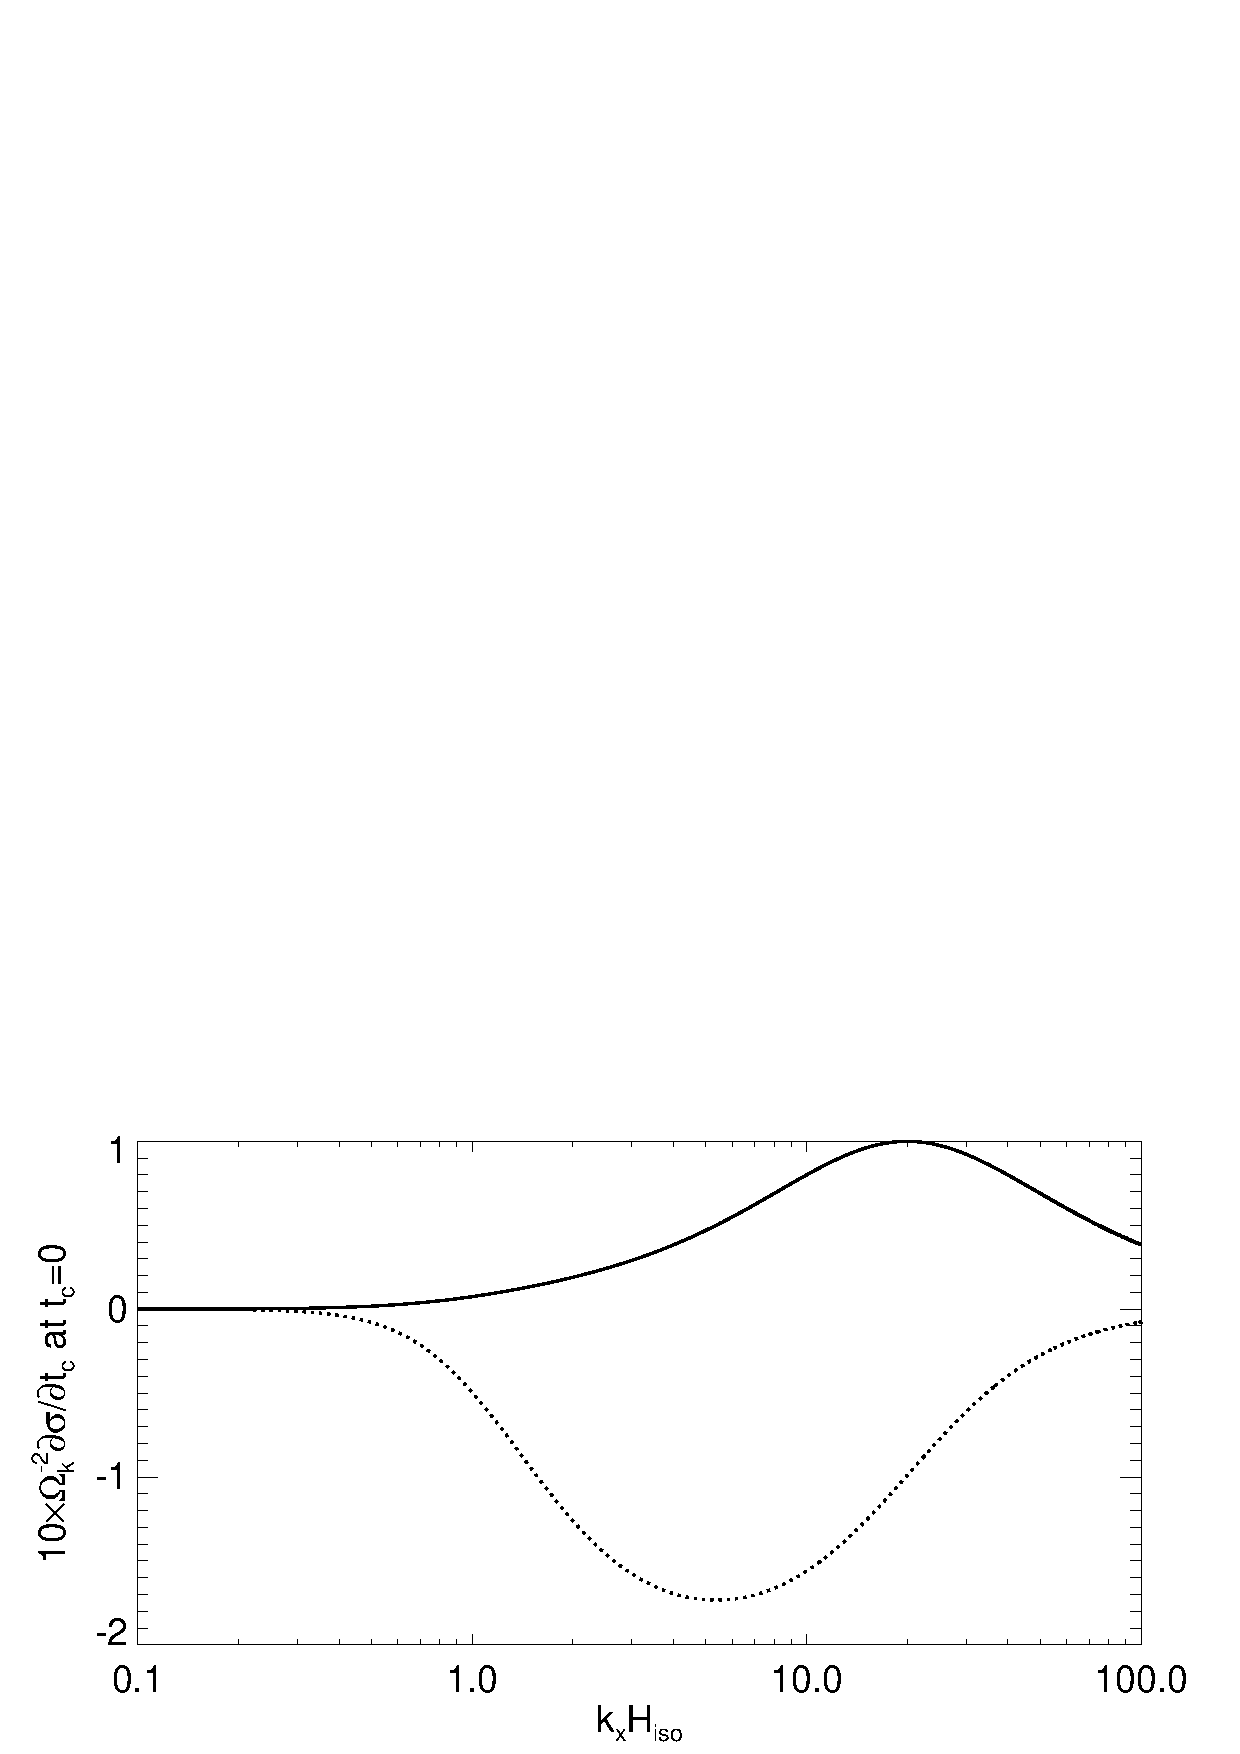
\includegraphics[width=\linewidth]{figures/domegadbeta}
  \caption{Rate of change of the fundamental VSI eigenfrequency
    $\sigma$ with respect to the introduction of a small but finite
    cooling time. The plotted quantity is $\p\hat{\sigma}/\p\beta$ at $\beta=0$, evaluated using
    Eq. \ref{nearly_iso_dsig} with 
    disk parameters $\epsilon=0.05$, $q=-1$ and $\gamma=1.4$. The real
    (imaginary) part of $\p\hat{\sigma}/\p\beta$ is shown as the solid
    (dotted) lines. 
    \label{domegadbeta}}  
\end{figure}   

One effect of introducing finite thermal relaxation is buoyancy. % We
% show in the next section that buoyancy strongly stabilizes the
% VSI.
The $\zhat^2$ depedence in $\delta v_{z1}$ then makes sense because it
is most significant for large $\zhat$, i.e. away from the midplane
where the effect of buoyancy first appears as $t_c$ is increased. 

\subsubsection{Dispersion relation with thermal relaxation}\label{disp_relax}
Eq. \ref{nearly_iso_explicit} is same form
as the governing equation for the adiabatic case
(Eq. \ref{adia_iso4}). However, the coefficients $\widetilde{B}$ and $\widetilde{C}$
have a complicated dependence on $\hat{\sigma}$. 
Applying the same solution method as in \S\ref{adia_explicit}, we 
% Thus calculating the
% eigenfrequency $\hat{\sigma}$ generally requires a numerical
% approach, which we do  in \S\ref{disp_relax}. However, analytical
% results may be obtained in the limit $\beta\to0$. 
find the adiabatic dispersion relation,
Eq. \ref{adia_disp0}, generalizes to a $6^\mathrm{th}$ order
polynomial in $\hat{\sigma}$ with finite thermal relaxation:
\begin{align}
  0 = \sum_{l=0}^{6}c_l\hat{\sigma}^l,\label{relax_disp}
\end{align}
where the coefficients $c_l$ are given in Appendix \ref{relax_coeff}.
Eq. \ref{relax_disp} contrasts to Eq. \ref{adia_disp}, which is
quadratic in $\hat{\sigma}$ for adiabatic perturbations. 

It is simplest to solve Eq. \ref{relax_disp} numerically. In
Fig. \ref{relax_disp_fig} we plot the growth rate of the fundamental
($M=0$) VSI mode as a function of $k_xH_\mathrm{iso}$ for a range of
dimensionless thermal relaxation timescales $\beta$, in a disk with
$\epsilon=0.05$, $q=-1$ and $\gamma=1.4$.  Similarly, 
in Fig. \ref{relax_bcrit} we solve the dispersion relation for the
critical $\beta$ such that the growth rate of the fundamental VSI mode
is zero.  

Fig. \ref{relax_disp_fig}---\ref{relax_bcrit} shows that a growing fundamental
VSI mode exists both in the isothermal ($\beta\to0$) and adiabatic
($\beta\to\infty$) limits, although the latter growth rates are
smaller by at least a factor of two. Furthermore, the adiabatic VSI is 
is limited to a thin layer about the disk midplane so it may be
considered stable. Then Fig. \ref{relax_bcrit} shows that 
$\beta\lesssim 0.1$ is required for instability in this disk model. This critical
timescale is indepedent of $k_x$ for
$k_xH_\mathrm{iso}\gtrsim10$. The top panel of Fig. \ref{relax_disp_fig} is also
consistent with the previous
discussion that show thermal relaxation has no effect for
$k_x\to0$ or $k_x\to\infty$ as $\beta\to0$. 

\begin{figure}
  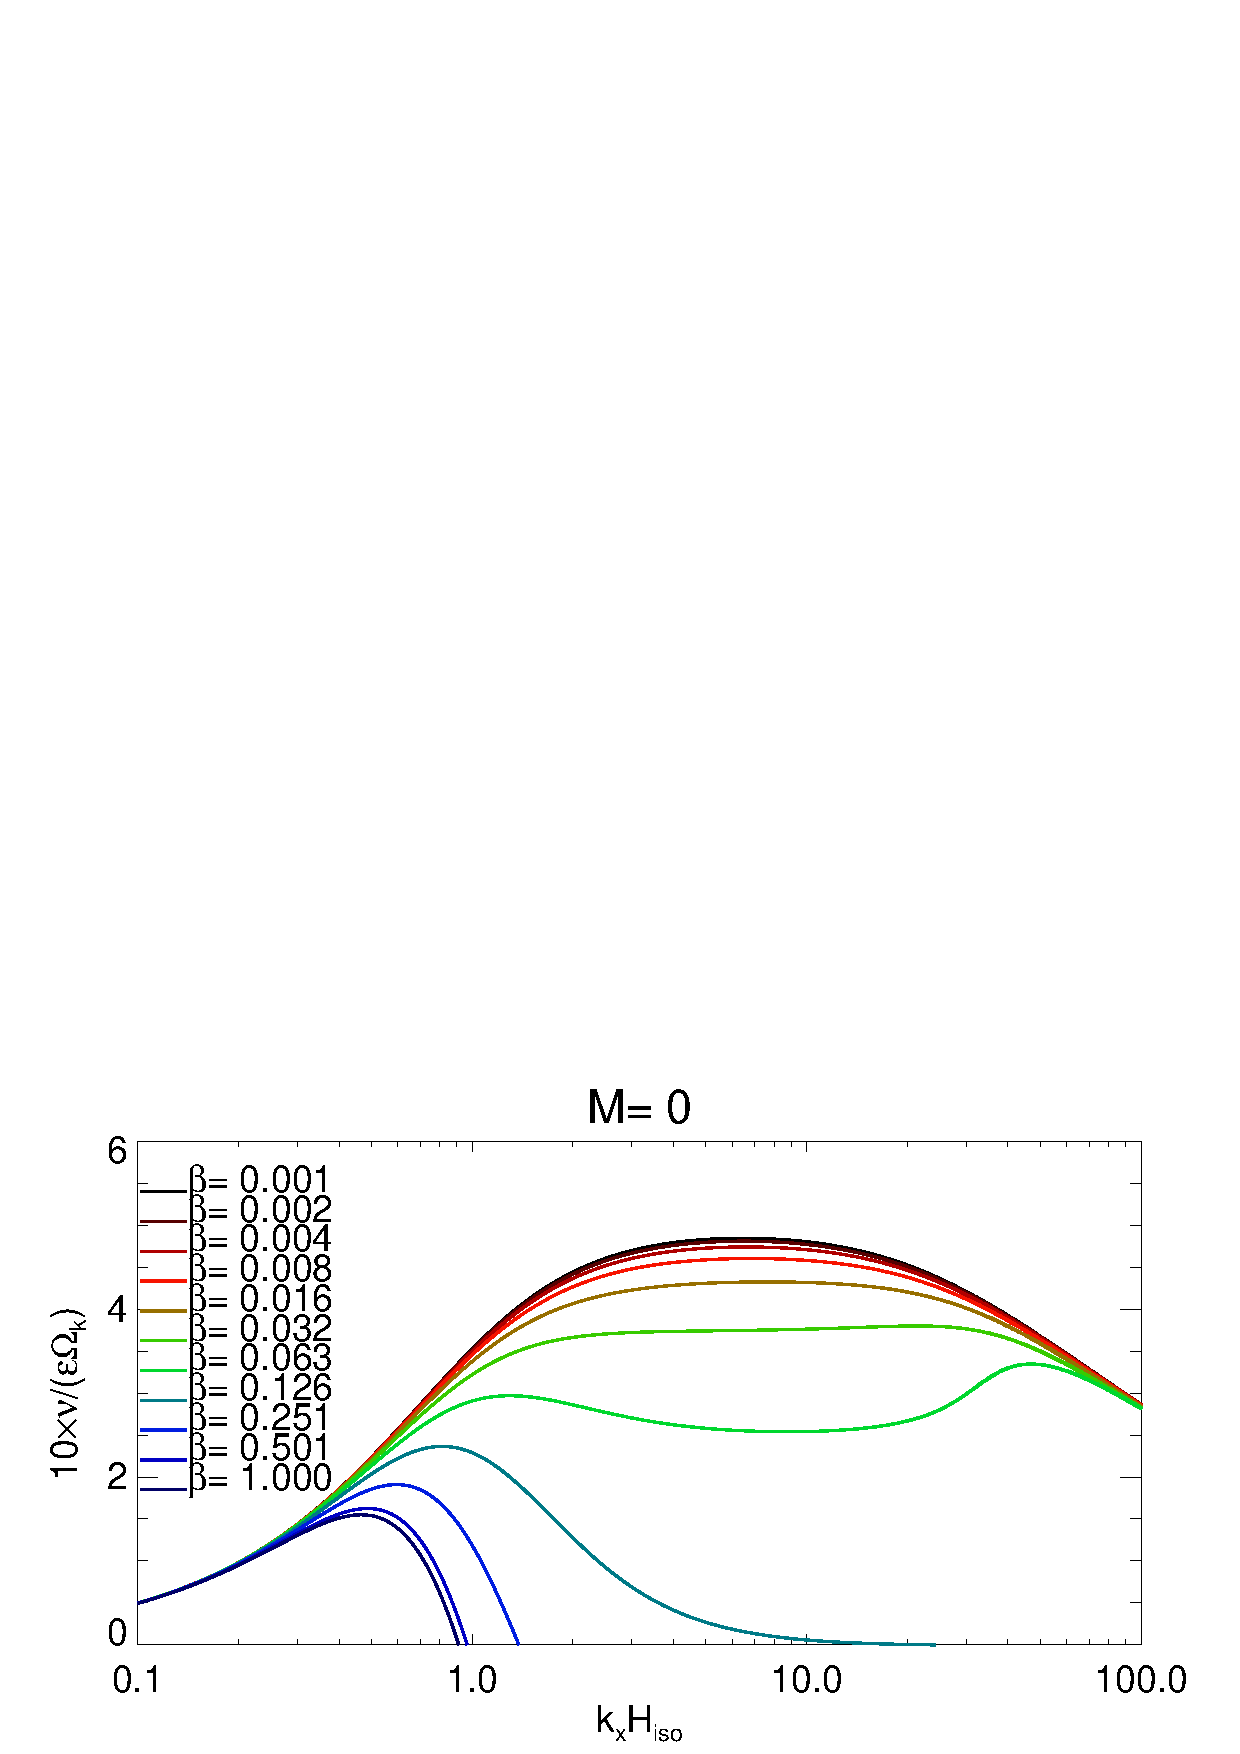
\includegraphics[width=\linewidth,clip=true,trim=0cm 1.75cm 0cm 0cm]{figures/rate_theory_grow_relax}
  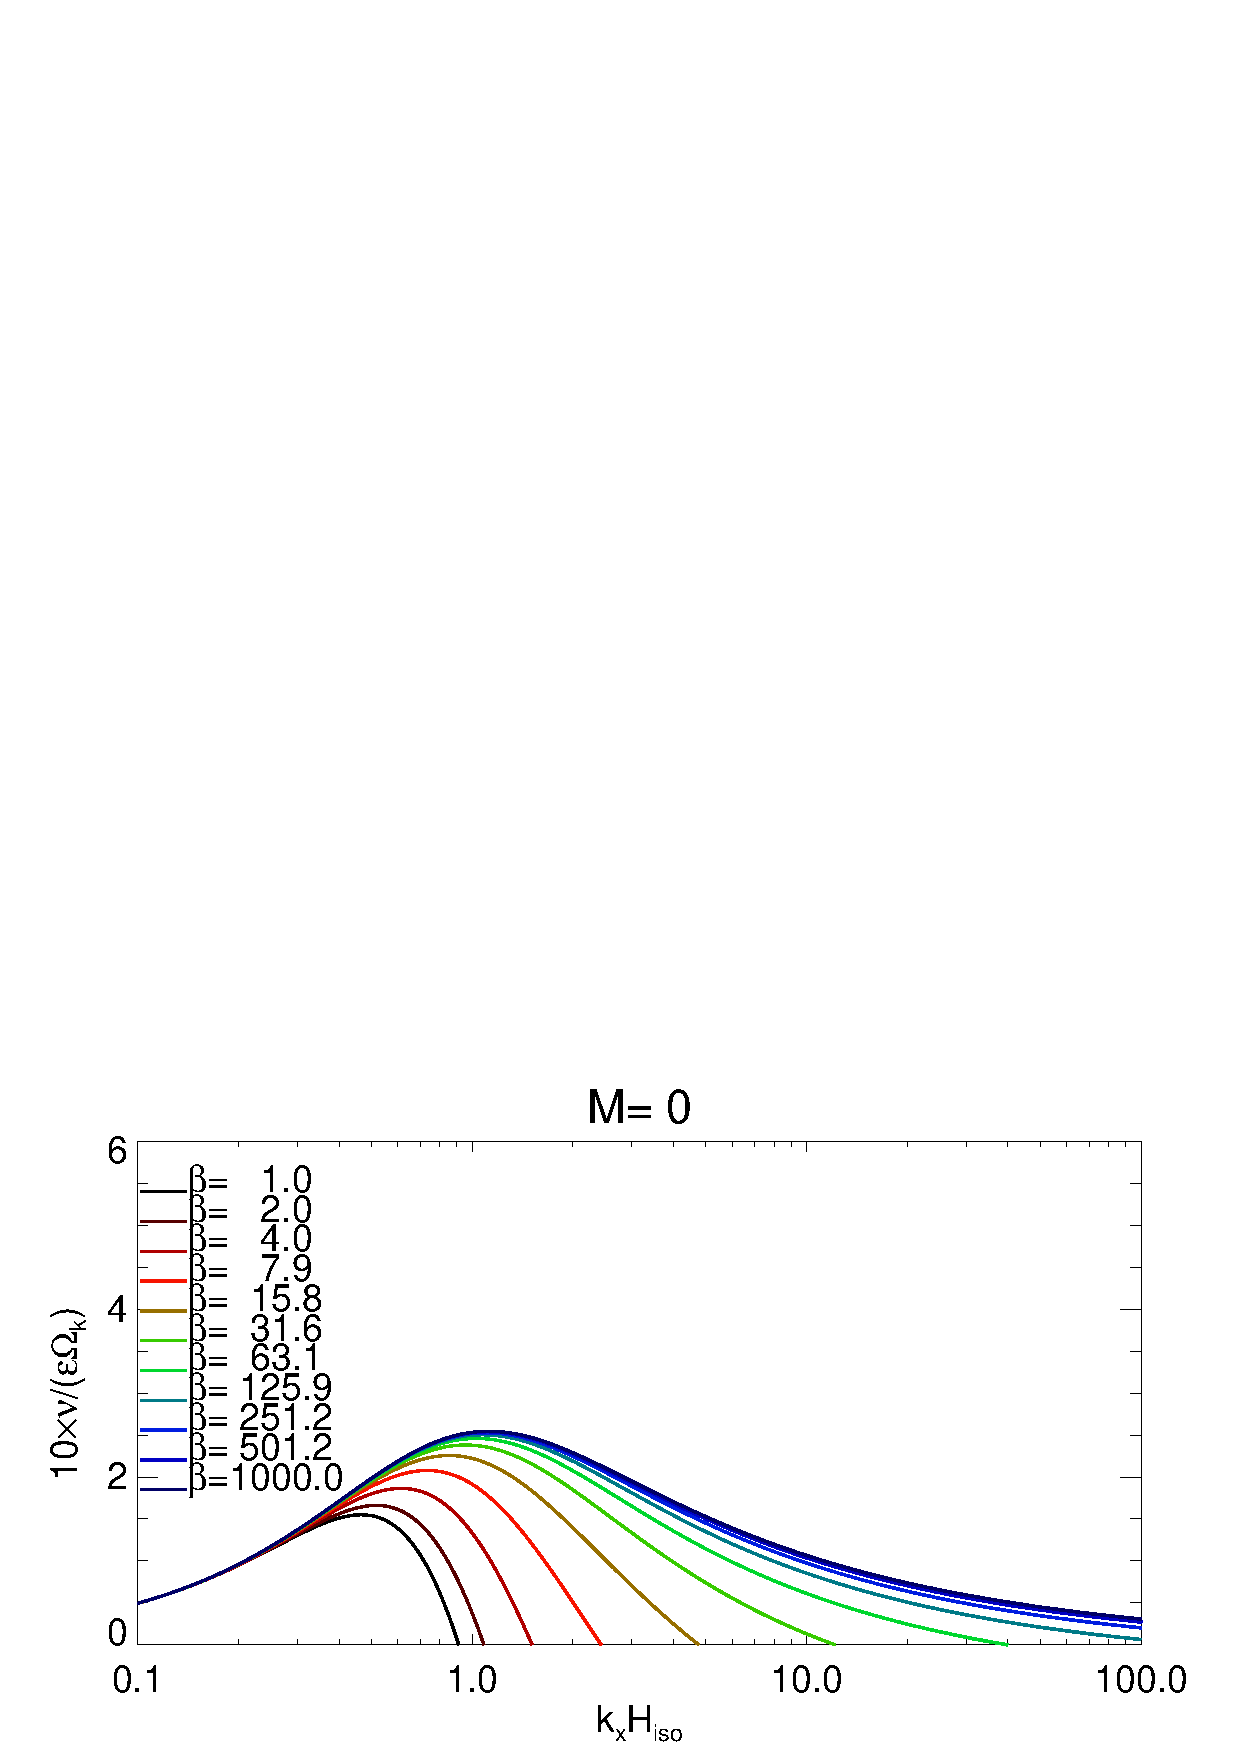
\includegraphics[width=\linewidth,clip=true,trim=0cm 0cm 0cm 1cm]{figures/rate_theory_grow_relax2}
  \caption{Growth rate of the fundamental VSI mode in a disk with
    dimensionless thermal relaxation timescales
    $\beta\in[10^{-3},1]$ (top) and $\beta\in[1,10^3]$ (bottom).
Other disk parameters are
    $\epsilon=0.05$, $q=-1$ and $\gamma=1.4$. The growth rates are
    calculated from the dispersion relation Eq. \ref{relax_disp}. 
    \label{relax_disp_fig}}  
\end{figure}   

%ate_theory, eps=0.05, smallq=-1d0, gmma=1.4, bmax=1.0, ncases=11,
%mmode=0.0, root=1, legend=[0.102,0.14,5.4,0.355], yrange=[0,6]

\begin{figure}
  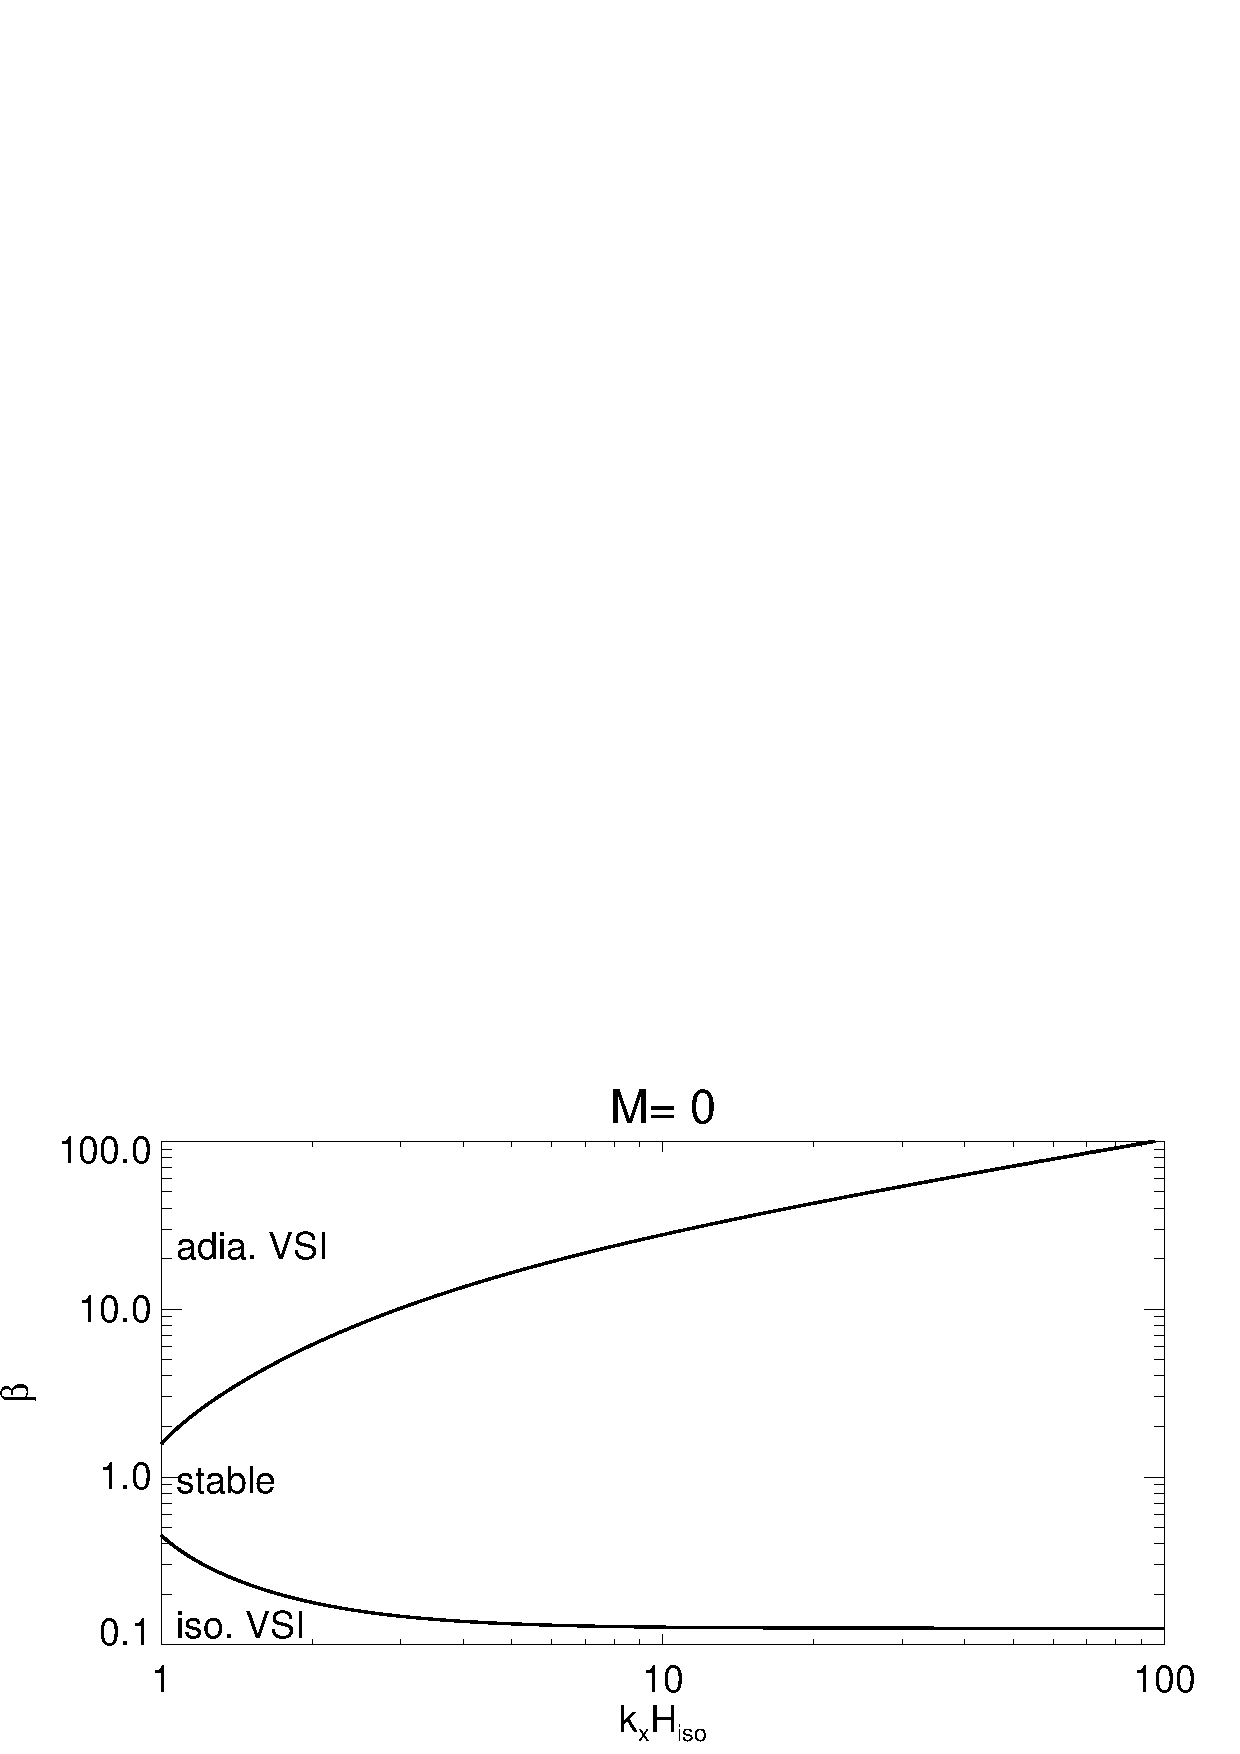
\includegraphics[width=\linewidth]{figures/bcrit_theory}
  \caption{Condition on the thermal relaxation timescale $\beta$ for the existence of unstable fundamental VSI
    modes in a vertically isothermal disk with $\epsilon=0.05$, $q=-1$
    and $\gamma=1.4$. For sufficiently small $\beta$ the isothermal VSI opertates,
    while for sufficiently large $\beta$ the adiabatic VSI
    operates. For intermediate values of $\beta$ the VSI growth rate
    is negative (i.e. stabilized). 
    \label{relax_bcrit}}  
\end{figure}   


\subsubsection{Upper limit on the thermal relaxation timescale for the
  fundamental isothermal VSI mode}\label{iso_vsi_beta_crit}
Notice in Fig. \ref{relax_bcrit} the upper limit on $\beta$ for the
fundamental isothermal VSI tends to a constant for large
$\khat$. Using this clue, we can calculate this critical $\beta$ by
considering $\khat\to\infty$. We proceed as follows. 

At marginal stability, the eigenfrequency $\hat{\sigma}=\hat{\omega}$
is real. The dispersion relation for the fundamental mode is then
\begin{align}\label{relax_disp_fund}
  0 = \sum_{l=1}^{6}c_l\hat{\omega}^l \quad \text{for $M=\hat{\nu}=0$}.  
\end{align} 
Taking the real and imaginary parts of Eq. \ref{relax_disp_fund} in
the limit $\khat\to\infty$ we find
\begin{align}
  0 =& \left[1 + \gamma\beta^2\left(1-\gamma\right)\right] + 2\epsilon q
  \gamma\beta (\hat{\omega}\khat) -  (\hat{\omega}\khat)^2 \notag\\
  &+ \beta^2\gamma^2\hat{\omega}^2 (\hat{\omega}\khat)^2,\label{relax_cond1}\\
  0=& \beta(1-\gamma)\khat^2 + \epsilon q \khat^2 (\hat{\omega}\khat)
  - 2\beta (\hat{\omega}\khat)^2 - \epsilon q \gamma^2\beta^2 (\hat{\omega}\khat)^3.\label{relax_cond2}
\end{align}
We seek solutions with
\begin{align}
  \khat \to \infty, \quad \hat{\omega}\to 0 ,\quad \khat\hat{\omega} \text{ finite}.
\end{align}
Then
\begin{align}
  \khat\hat{\omega} = \frac{(\gamma-1)\beta}{\epsilon q}
\end{align}
from Eq. \ref{relax_cond2}, which implies, from Eq. \ref{relax_cond1}
that
\begin{align}
  \beta = \frac{1}{(\gamma-1)}\left[\frac{1}{\left(\epsilon
        q\right)^2} - \frac{\gamma}{(\gamma-1)}\right]^{-1/2}. 
\end{align}
For a thin disk $\epsilon\ll 1$, we infer 
\begin{align}\label{iso_vsi_cond}
  \beta \lesssim \frac{|\epsilon q|}{\gamma-1} \equiv
  \beta_\mathrm{crit} 
\end{align}
is required for the fundamental isothermal VSI to operate.  For
$\epsilon = 0.05$, $q=-1$ and $\gamma=1.4$ we find
$\beta_\mathrm{crit}=0.125$, in agreement with Fig. \ref{relax_bcrit}
at large $\khat$. 

\subsubsection{Lower limit on the thermal relaxation timescale for the
  fundamental adiabatic VSI mode}
{\bf Note: for reference only. Not to be included in paper.} 
Fig. \ref{relax_bcrit} indicates there exists a lower limit on the
thermal relaxation time for the system to behave adiabatically and
support the fundamental adiabatic VSI. This critical
timescale satisfies Eq. \ref{relax_cond1}---\ref{relax_cond2} with 
\begin{align}
  \beta \sim \beta_0\khat^{1/2},\quad \hat{\omega}  \sim
  \hat{\omega}_0\khat^{-1/2} \text{ as } \khat\to\infty.
\end{align}
The constants $\beta_0$ and $\hat{\omega}_0$ are determined by the
simultaneous equations
\begin{align}
  & 0 = \gamma\beta_0^2(1-\gamma) + 2\epsilon q \gamma
  \beta_0\hat{\omega}_0 - \hat{\omega}_0^2 +
  \beta_0^2\gamma^2\hat{\omega}_0^4.\\
  & 0= \beta_0(1-\gamma) + \epsilon q \hat{\omega}_0 - \epsilon q
  \gamma^2 \beta_0^2\hat{\omega}_0^3. 
\end{align}
For $\epsilon = 0.05$, $q=-1$ and $\gamma=1.4$, the appropriate
solution is $\beta_0 = 10.33$ and $\hat{\omega}_0 = 0.74$.  


% The pair of ODEs for $W$ and $Q$
% (Eq. \ref{ode_w}---\ref{ode_Q}) with these approximations and 
% written with dimensionless variables, are
% \begin{align}
%   &\hat{\sigma}^2\left(Q +  \hat{k}^2W\right) \notag\\ 
%   &= \hat{z} \left(1 +
%     \ii\epsilon q \hat{k} \right)\left[W^\prime - \zhat \left(W -
%       Q\right)\right] - \left[W^\prime - \zhat \left(W -
%       Q\right)\right]^\prime\label{nearly_iso1},\\
% &\beta \hat{\sigma}^2\left(W - \gamma Q\right) + \ii\hat{\sigma}
%     \left(W-Q\right)\notag\\
%    & = -\beta\zhat\left(\gamma-1\right) \left[W^\prime - \zhat \left(W -
%       Q\right)\right]\label{nearly_iso2},
% \end{align}
% where we recall $\beta = t_c\Omega_k$ is the dimensionless cooling
% time. It is evident that for $\beta\equiv 0$, we recover
% Eq. \ref{iso_ode3}. In addition, from the expression of the vertical
% velocity perturbation (Eq. \ref{lin_vz}) we have
% \begin{align}
%   W^\prime - \zhat \left(W -
%       Q\right) = \ii\hat{\sigma}c_s\delta v_z. \label{nearly_vz}
% \end{align}

% %is valid for
% %non-isothermal perturbations $\gamma>1$ if the thermal relaxation
% %(cooling) timescale $t_c\equiv0$. 


% % Then we may linearize Eq. \ref{nearly_iso1}---\ref{nearly_iso2} 

% To determine the (assumed) small effect of introducing a short thermal
% relaxation, we linearize Eq. \ref{nearly_iso1}---\ref{nearly_iso2} about a known
% solution for $\beta\equiv0$. Let 
% \begin{align}\label{nearly_iso_pert}
%   \beta \to 0 + \delta\beta,\, W\to W+\delta W,\, Q \to Q+\delta
%   Q,\,\hat{\sigma} \to \hat{\sigma} + \delta\hat{\sigma}, 
% \end{align} 
% where $W=Q$ is the polynomial solution described in \S\ref{iso_poly}
% with $\hat{\sigma}^2$ given by Eq. \ref{sig2_iso}. Inserting
% Eq. \ref{nearly_iso_pert} into
% Eq. \ref{nearly_iso1}---\ref{nearly_iso2} and keeping only first order
% terms, we obtain
% \begin{align}
%   &2\hat{\sigma}\delta\hat{\sigma}\left(1+\hat{k}^2\right)W +
%   \hat{\sigma}^2 \left(\delta Q + \hat{k}^2\delta W\right)\notag\\
%   &= \zhat \left(1+\ii\epsilon q \hat{k}\right)\left[\delta W^\prime -
%     \zhat \left(\delta W - 
%       \delta Q\right)\right] - \delta W^{\prime\prime}\notag\\
%   &\phantom{=} + \left[\zhat \left(\delta W -
%      \delta Q\right)\right]^\prime,\label{nearly_iso3}\\
% &\ii\hat{\sigma} \left(\delta W - \delta Q\right) =
% \delta\beta\left(\gamma-1\right)\left(\hat{\sigma}^2W - \hat{z}W^\prime\right).\label{nearly_iso4}
% \end{align}
% This is a pair of inhomogeneous ODEs with a forcing by $W$. The
% homogeneous problem is, of course, just the ODE for $\beta=0$ solved
% in \S\ref{iso_poly}. Hence we only seek the particular solution. 

% We could proceed by considering the entire set of polynomial
% solutions for $W$, but it is simplest to look at the fundamental
% mode. Thus we consider the `basic state' 
% \begin{align*}
%   W = \hat{z},\quad \hat{\sigma}^2\left(1+\hat{k}^2\right) = 1 +
%   \ii\epsilon q \hat{k},
% \end{align*}
% then
% \begin{align}
%   \delta W = b \zhat^3,
% \end{align}
% where $b$ is a constant to be determined. Eliminating $\delta Q$ from
% Eq. \ref{nearly_iso3}---\ref{nearly_iso4}, inserting the above
% expressions for $W$ and $\delta W$ and balancing coefficients of
% $\zhat$ and $\zhat^3$, we find
% \begin{align}
%  & 2\left(1+\ii\epsilon q \hat{k}\right) \delta\hat{\sigma} \notag\\& = -6b\hat{\sigma} -
% 2\ii \delta \beta\left(\gamma-1\right)\left(\hat{\sigma}^2-1\right) - \ii
%   \hat{\sigma}^2\delta\beta\left(\gamma-1\right),\\
% & 0=  2b\hat{\sigma}+\ii\delta\beta
% \left(\gamma-1\right)\left(\hat{\sigma}^2 - 1\right),
% \end{align}
% where the expression for $\hat{\sigma}^2$ was used.
